\documentclass[border=5pt]{standalone}
\usepackage{tikz}
\usepackage{amsmath}
\usetikzlibrary{arrows.meta, positioning, calc}

\begin{document}
\begin{tabular}{@{}c@{\hspace{12mm}}|@{\hspace{12mm}}c@{\hspace{12mm}}|@{\hspace{12mm}}c@{}}
\textbf{Early Injection} & \textbf{FiLM} & \textbf{Cross-Attention} \\[6pt]
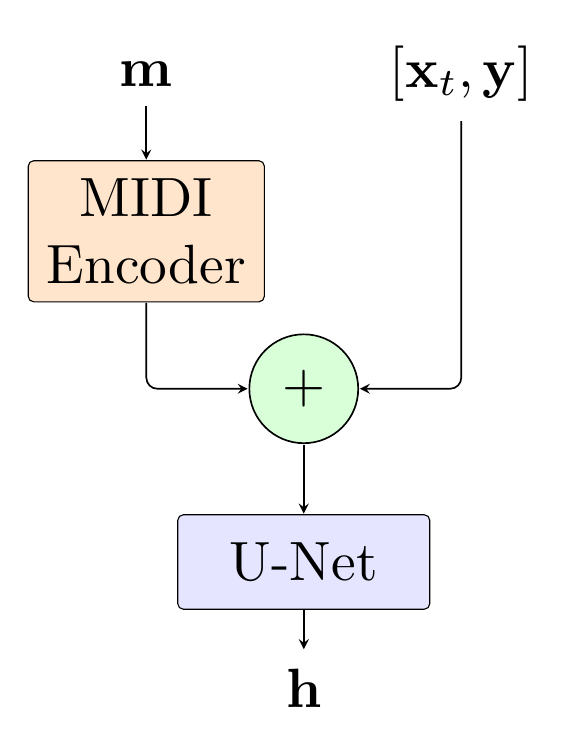
\begin{tikzpicture}[scale=2, transform shape, font=\normalsize, baseline=(current bounding box.north),
  unetbox/.style = {draw, rounded corners=2pt, minimum width=16mm, minimum height=6mm, align=center, fill=blue!10},
  plusbox/.style = {circle, draw, minimum size=5mm, align=center, fill=green!15, semithick},
  encoderbox/.style = {draw, rounded corners=2pt, minimum width=14mm, minimum height=5mm, align=center, fill=orange!20},
  arrow/.style = {->, >=stealth, semithick}
]
\node (m_raw) at (-10mm,17mm) {$\mathbf{m}$};
\node (xt) at (10mm,17mm) {$[\mathbf{x}_t, \mathbf{y}]$};
\node[encoderbox] (encoder) at (-10mm,7mm) {MIDI\\Encoder};
\node[plusbox] (plus2) at (0,-3mm) {$+$};
\node[unetbox] (unet) at (0,-14mm) {U-Net};
\node (out) at (0,-22mm) {$\mathbf{h}$};
\draw[arrow] (m_raw) -- (encoder);
\draw[arrow, rounded corners=4pt] (encoder.south) -- (encoder.south |- plus2.west) -- (plus2.west);
\draw[arrow, rounded corners=4pt] (xt.south) -- (xt.south |- plus2.east) -- (plus2.east);
\draw[arrow] (plus2) -- (unet);
\draw[arrow] (unet) -- (out);
\end{tikzpicture}
&
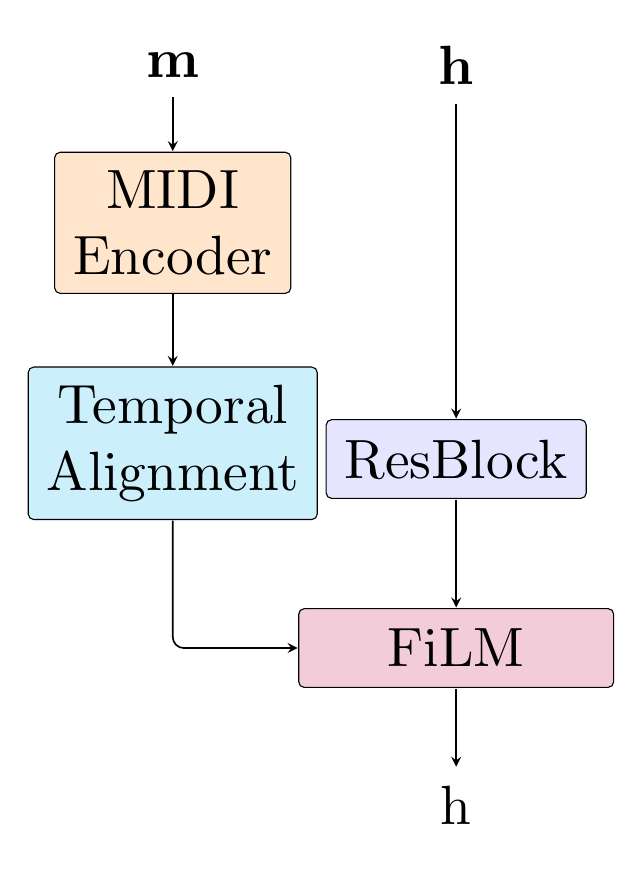
\begin{tikzpicture}[scale=2, transform shape, font=\normalsize, baseline=(current bounding box.north),
  box/.style = {draw, rounded corners=2pt, minimum width=16mm, minimum height=5mm, align=center},
  filmbox/.style = {draw, rounded corners=2pt, minimum width=20mm, minimum height=5mm, align=center},
  cubebox/.style = {draw, minimum width=12mm, minimum height=5mm, align=center, fill=gray!10, rounded corners=2pt,
    path picture={
      \draw[fill=gray!20] (path picture bounding box.north east) -- ++(1.5mm,1.5mm) -- ++(0,-5mm) -- (path picture bounding box.south east) -- cycle;
      \draw[fill=gray!15] (path picture bounding box.north east) -- ++(1.5mm,1.5mm) -- ++(-12mm,0) -- (path picture bounding box.north west) -- cycle;
    }},
  arrow/.style = {->, >=stealth, semithick}
]
\node (h_input) at (0,5mm) {$\mathbf{h}$};
\node (midi_input) at (-18mm,5mm) {$\mathbf{m}$};
\node[cubebox, fill=orange!20] (midi_encoder) at (-18mm,-5mm) {MIDI\\Encoder};
\node[box, fill=cyan!20] (temporal_align) at (-18mm,-19mm) {Temporal\\Alignment};
\node[box, fill=blue!10] (resblock) at (0,-20mm) {ResBlock};
\node[filmbox, fill=purple!20] (film) at (0,-32mm) {FiLM};
\node (output) at (0,-42mm) {h};
\draw[arrow] (h_input) -- (resblock);
\draw[arrow] (resblock) -- (film);
\draw[arrow] (film) -- (output);
\draw[arrow, rounded corners=4pt] (temporal_align.south) |- (film);
\draw[arrow] (midi_input) -- (midi_encoder);
\draw[arrow] (midi_encoder) -- (temporal_align);
\end{tikzpicture}
&
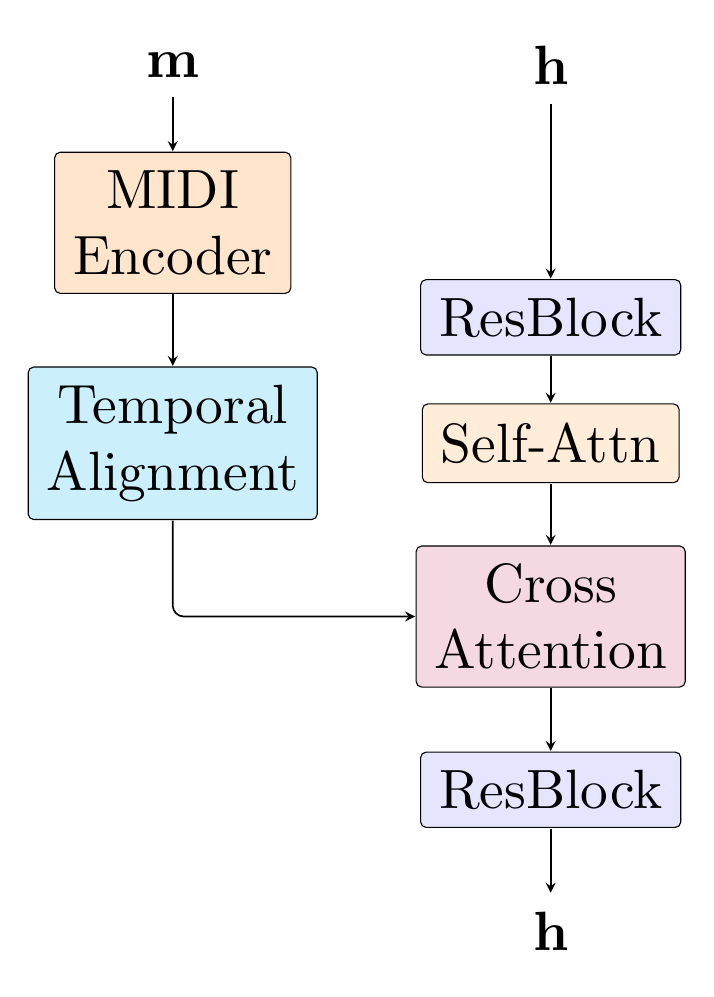
\begin{tikzpicture}[scale=2, transform shape, font=\normalsize, baseline=(current bounding box.north),
  resbox/.style = {draw, rounded corners=2pt, minimum width=14mm, minimum height=4mm, align=center, fill=blue!10},
  crossbox/.style = {draw, rounded corners=2pt, minimum width=16mm, minimum height=5mm, align=center, fill=purple!15},
  selfbox/.style = {draw, rounded corners=2pt, minimum width=16mm, minimum height=5mm, align=center, fill=orange!15},
  encoderbox/.style = {draw, rounded corners=2pt, minimum width=10mm, minimum height=4mm, align=center, fill=orange!20},
  alignbox/.style = {draw, rounded corners=2pt, minimum width=10mm, minimum height=4mm, align=center, fill=cyan!20},
  arrow/.style = {->, >=stealth, semithick}
]
\node (h_in) at (0,28mm) {$\mathbf{h}$};
\node[resbox] (res1) at (0,12mm) {ResBlock};
\node[selfbox] (self) at (0,4mm) {Self-Attn};
\node[crossbox] (cross) at (0,-7mm) {Cross\\Attention};
\node[resbox] (res2) at (0,-18mm) {ResBlock};
\node (h_out) at (0,-27mm) {$\mathbf{h}$};
\node (m_raw) at (-24mm,28mm) {$\mathbf{m}$};
\node[encoderbox] (midi_encoder) at (-24mm,18mm) {MIDI\\Encoder};
\node[alignbox] (temporal_align) at (-24mm,4mm) {Temporal\\Alignment};
\draw[arrow] (h_in) -- (res1);
\draw[arrow] (res1) -- (self);
\draw[arrow] (self) -- (cross);
\draw[arrow] (cross) -- (res2);
\draw[arrow] (res2) -- (h_out);
\draw[arrow] (m_raw) -- (midi_encoder);
\draw[arrow] (midi_encoder) -- (temporal_align);
\draw[arrow, rounded corners=4pt] (temporal_align.south) |- (cross.west);
\end{tikzpicture}
\end{tabular}
\end{document}
